\documentclass[10pt,a4paper]{article}
\usepackage[left=1.5cm,right=1.5cm,top=1.5cm,bottom=1.5cm]{geometry}
\usepackage[utf8]{inputenc}
\usepackage[german]{babel}
\usepackage{amsmath}
\usepackage{amsfonts}
\usepackage{amssymb}
\usepackage{amsthm}
\usepackage{graphicx}

\newenvironment{packed_enum}{
\begin{enumerate}
  \setlength{\itemsep}{1pt}
  \setlength{\parskip}{0pt}
  \setlength{\parsep}{0pt}
}{\end{enumerate}}
\newcommand{\abs}[1]{\ensuremath{\left\vert#1\right\vert}}
\begin{document}
\section{Allgemeines}
\subsection{Nabla Operator $\nabla$}
\[
\vec{\nabla} = \left(\frac{\partial}{\partial x_1}, ..., \frac{\partial}{\partial x_n} \right)
\,\,\,\,\,\,\,\,\,\,\,\,\,\,\,\,\,\,\,\,\,\,\,\,\,\,\,\,
\vec{\nabla} \vec{V} = \sum\limits_{i=1}^n \frac{\partial V_i}{\partial x_i}
\]

\section{Partielle Differentialgleichungen}
\subsection{Homogene lineare partielle Differentialgleichungen 1. Ordnung}
\begin{packed_enum}
\item Umstellen in Normalform: $\sum\limits_{i = 1}^n a_i(\vec{x}) \cdot u_i = 0$, weitere Beispiele für $n=2$.
\item Charakteristische DGLs sind zu lösen: $\dot{x}(t) = a_1(x(t), y(t)); \dot{y}(t) = a_2(x(t), y(t))$
\begin{packed_enum}
\item Dabei darf man alle Gleichungen z.B. durch eine andere teilen
\item Hat man dies getan, erhält man z.B. $\dot{x}(t)=1$ und somit $x(t)=t+c$ und $c=0$ ist zulässig, also $x=t$
\end{packed_enum}
\item Eine der Gleichungen durch Variablen der anderen darstellen: $y = \psi(x, C)$, nach $C(\vec{c})$ umstellen $C(\vec{c}) = \phi(x,y)$
\item $\Phi(\phi(x,y))$ mit beliebigem $\Phi$ aus $C^1$ ist die Lösung
\item Allgemein: $u(\vec{x}) = \Phi(\phi_1({x}), ... , \phi_{n-1}(\vec{x}))$
\end{packed_enum}

\subsection{Quasilineare partielle inhomogene Differentialgleichungen 1. Ordnung}
So sieht sie aus: $\sum\limits_{i=1}^n a_i(\vec{x}, u)\cdot u_{x_i} = b(\vec{x}, u)$

Lösen mit erweiterter quasilinearer homogener DGL: $\left( \sum\limits_{i=1}^n a_i(\vec{x}, u)\cdot U_{x_i} \right) + b(\vec{x}, u)\cdot U_u = 0$ und $U = 0$

Dann wie homogene lineare partielle Differentialgleichungen 1. Ordnung lösen.

Zum Schluss eine Basis als Funktion der anderen Basis darstellen, nach $u$ umformen und $\psi(...)$ passend aussuchen.

\subsection{Anfangswertaufgaben}
$u(\vec{x}) = \Phi(\phi_1({x}), ... , \phi_{n-1}(\vec{x}))$

Anfangsfunktion: $u_0(s) := u(x(s), y(s))$ auf der Kurve $c(s) := (x(s), y(s))^T$.

\subsection{Burgersgleichung}
TODO

\subsection{Lineare inhomogene partielle Differentialgleichungen 2. Ordnung}
\[
\sum\limits_{i,j=1}^n a_{ij}(\vec{x})u_{x_ix_j} + \sum\limits_{i=1}^n b_i(\vec{x}) u_{x_i} + f(\vec{x})u = g(\vec{x})
\]

Für $n=2$ und $\vec{x}=(x,y)$: $au_{xx} +2bu_{xy}+cu_{yy} + du_x+eu_y+fu=g$

Matrix: $
\left(
\begin{matrix}
a & b \\
b & c \\
\end{matrix}
\right)
TODO
$

TODO typen und kriterien aufschreiben. Fuer $n=2$ immer det nehmen, ultrahyperbolisch gibts nur in hoehreren Dimensionen.

3 Dim: $au_{xx}+2bu_{xy}+2cu_{xz}+2du_{yz}+eu_{yy}+fu_{zz}+gu_x +hu_y+iu_z+ju=k$

$\nabla^T
\begin{pmatrix}
a & b&c \\
b & e&d \\
c&d&f\\
\end{pmatrix}
\nabla u+\left(g - \nabla^T \begin{pmatrix}
a\\b\\c\\
\end{pmatrix}, h - \nabla^T \begin{pmatrix}
b\\e\\d\\
\end{pmatrix},i - \nabla^T \begin{pmatrix}
e\\d\\f\\
\end{pmatrix}\right)\nabla u + ju = k$

\section{Polarkoordination}
\subsection{Produktansatz in Polarkoordinaten}
$(x,y) = (r\,cos \phi, r\, sin \phi) \Rightarrow u_{rr} + \frac{u_r}{r} + \frac{u_{\phi\phi}}{r^2}$

\pagebreak
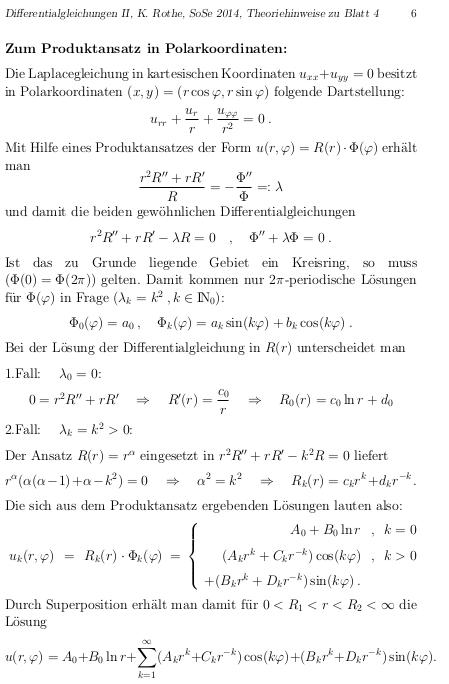
\includegraphics[scale=1]{ununderstandable}
\end{document}
